\section{Models of digital systems in \hilecop{}}
\label{sec:hilecop-models}

Let us introduce the input formalism of \hilecop{}'s model-to-text
transformation: Synchronously executed, extended, generalized,
Interpreted Time Petri Nets with priorities (SITPNs). The
formalization of the SITPN structure and semantics is mainly the
result of two Ph.D. theses \cite{Leroux2014,Merzoug2018}. We made a
preciser definition of both the SITPN structure and its semantics, as
precision is needed for proving semantic preservation. We have
implemented both structure and semantics in
\coq{}\footnote{\url{https://github.com/viampietro/ver-hilecop/tree/master/sitpn}}. Moreover,
we added complementary definitions, concerning the well-definition of
an SITPN input model, that are required to express our semantic
preservation theorem. In this section, we assume that the reader has
some knowledge of the Petri net formalism and its semantics, so that
words like firing, or marking, need no explanation. For more
information on the topic of Petri nets, the reader can refer to
\cite{David1994}, \cite{Murata1989}, or \cite{Diaz2001}.

\begin{figure}[H]
\centering
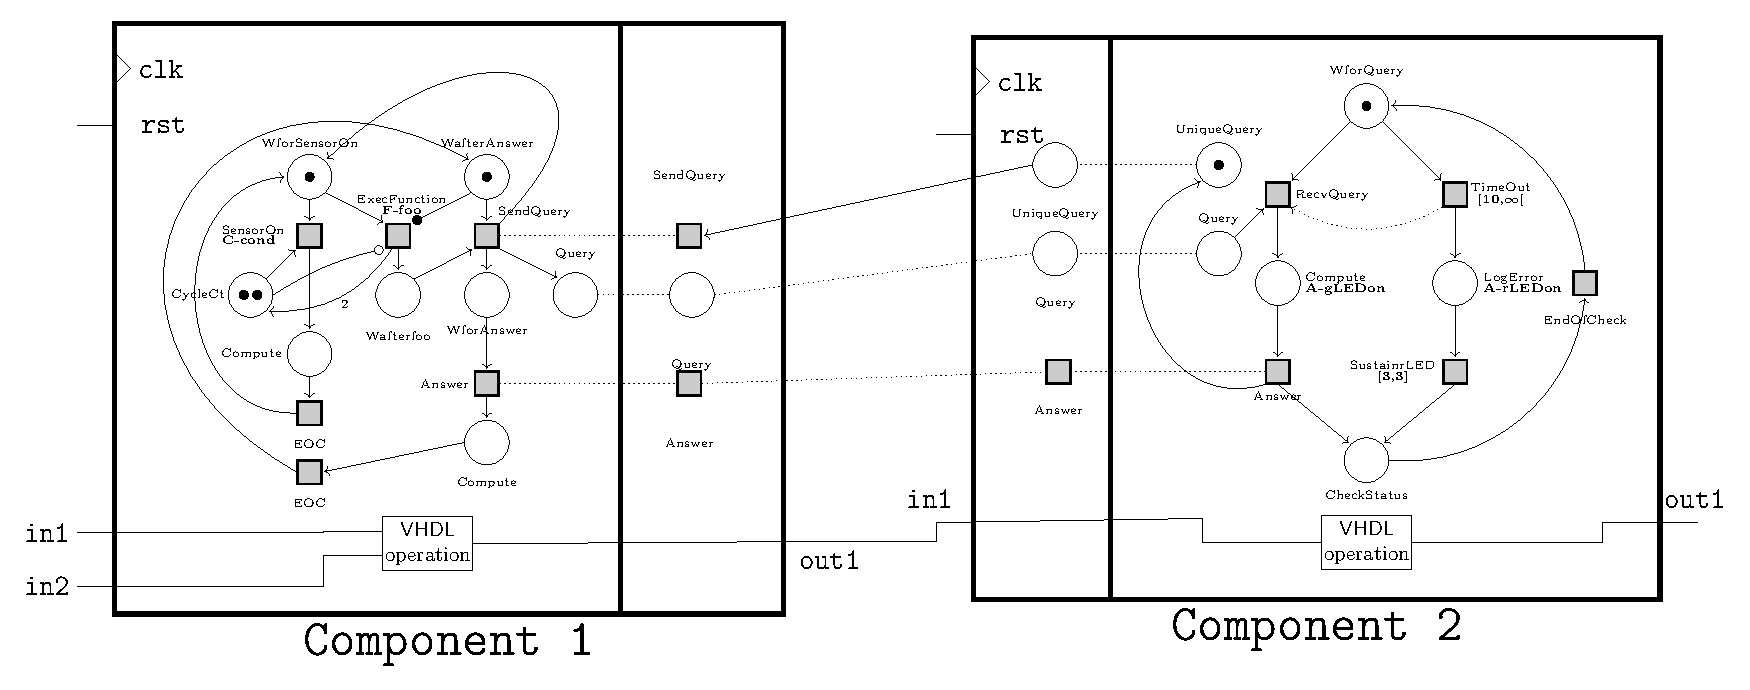
\includegraphics[keepaspectratio=true,width=\textwidth]{abs-model.eps}
\caption[An example of model of digital system in \hilecop{}.]{A
  component-based model of digital system in \hilecop{}.}
\label{fig:abs-model}
\end{figure}

In \hilecop{}'s high-level formalism, a model of digital system is
composed of boxes that represent the different components of the
system. Figure~\ref{fig:abs-model} gives an example of such a model.
The internal behavior of each component is defined by a SITPN model.
The elements of a component's internal behavior can be connected to
the elements of another component's behavior through an interface. Two
elements are either connected through a place-transition (or
transition-place) arc, or through a fusion arc (dotted line in
Figure~\ref{fig:abs-model}). While designing a component, an engineer
can also define input and output ports in the component interface,
declare internal signals, and perform operations over the ports and
internal signals by writing \vhdl{} code. All the \vhdl{} code defined
in this way will be copied as is in the output \vhdl{} design during
the model-to-text transformation. Note that all components declare a
clock and a reset signal (cf. \texttt{clk} and \texttt{rst} in
Figure~\ref{fig:abs-model}). These signals are related to the
synchronous execution of the system in the final physical device.

Before being transformed into \vhdl{} code, the model is flattened
down (cf. Step \circled{1} to step \circled{2} in
Figure~\ref{fig:hilecop-wf}). All component structures are removed,
and the result is one global SITPN model. During this flattening step,
all elements that were connected through fusion arcs are merged
together. Figure~\ref{fig:impl-model} presents the global SITPN model
resulting from the flattening of the component-based model of
Figure~\ref{fig:abs-model}.

\begin{figure}[H]
\centering
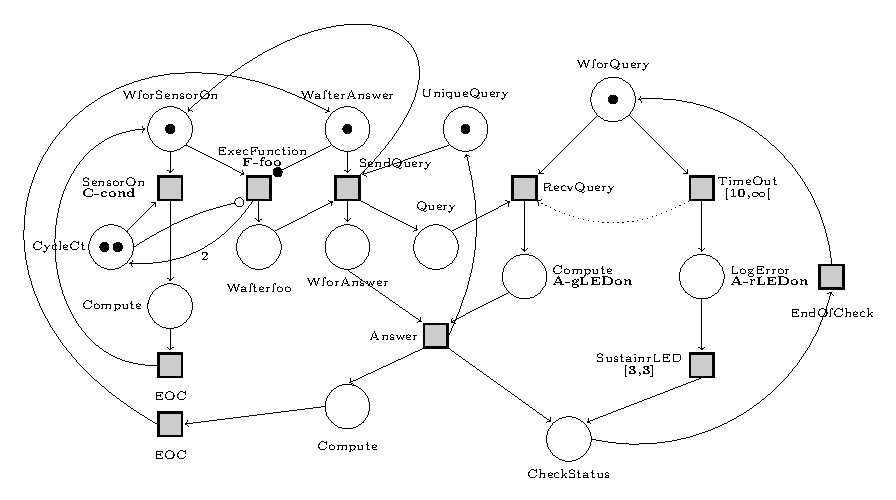
\includegraphics[keepaspectratio=true,width=\textwidth] {impl-model.eps}
\caption[Global Petri net model.]{A global Petri net model obtained
  after the flattening of a \hilecop{} high-level model.}
\label{fig:impl-model}
\end{figure}

SITPNs are a combination of multiple classes of PNs, namely: extended
PNs, generalized PNs, interpreted PNs, time PNs and PNs with
priorities. A generalized Petri net admits the weight of its arcs to
be a natural number instead of the default value of one (i.e. when no
number is written above the arc). An extended Petri net introduces two
kind of place-transition arcs, the \textit{inhibitor} arc,
characterized by a white circle head, and the \textit{test} arc, which
has a black circle head. These arcs add conditions the firing of a
connected transition, however, they do not cause tokens to be removed
from input places at firing time. In Figure~\ref{fig:impl-model}, the
arc from place CycleCt to transition ExecFunction is an inhibitor arc,
and the arc from place WafterAnswer to ExecFunction is a test arc.
Now, let us introduce more specifically the class of interpreted PNs,
time PNs and PNs with priorities.

\paragraph{Interpreted Petri nets (IPNs)}
% As stated in \cite{David1994}, Interpreted Petri Nets (IPN) ``can be
% applied to various interpretations according to the use wished to be
% made of it''.
In its general definition \cite{David1994}, an IPN is associated with
a finite set of variables $V$, a finite set of operations $O$, and a
finite set of conditions $C$. Operations of the $O$ set are associated
with places and triggered when the places become marked. The execution
of operations affects the value of the variables, and the value of
conditions depends on Boolean expressions computed upon the variables.
Conditions are associated with transitions and become involved in the
firing process.  In the \hilecop{} version of
IPNs, % refines the concepts of the general
% definition. In this version, 
the set of variables corresponds to the set of \vhdl{} signals that
are handled by the model; a signal can be an input port, an output
port or an internal signal of the modeled hardware circuit. The
operations, implemented by \vhdl{} procedures, are separated in two
kinds, namely: actions and functions. Actions (or continuous
operations) are associated to the places; all the actions associated
to a place $p$ are activated as long as $p$ is marked (i.e. as long as
$p$ holds a token). Functions (or discrete operations) are associated
to the transitions; when a transition $t$ is fired, all functions
associated to $t$ are executed once. In Figure \ref{fig:impl-model},
\textbf{C-cond} is a condition associated to the transition SensorOn;
\textbf{F-foo} is a function associated to the transition
ExecFunction; \textbf{A-gLEDon} and \textbf{A-rLEDon} are two actions
associated to the Compute and LogError places.

\paragraph{Time Petri nets (TPNs)}

In a TPN, time intervals can be associated to transitions, along with
a dynamic time counter value. Thus, the firing of a transition must
happen in a certain time window. In the \hilecop{} version of TPNs,
time intervals are of the form $[a, b]$, where $a\in\mathbb{N}^{*}$
and $b\in\mathbb{N}^{*}\sqcup\{\infty\}$.  In
Figure~\ref{fig:impl-model}, transitions SustainrLED and TimeOut are
both associated with time intervals.

\paragraph{Petri nets with priorities}

Two transitions are in structural conflict if they have a common input
place connected through a \textit{basic} arc (i.e. neither inhibitor
nor test arc). When two transitions in structural conflict are firable
at the same time and if the firing of one of the transitions disables
the other, then, the conflict becomes \textit{effective}. In a Petri
net with priorities, it is possible to specify a firing priority in
the case where the conflict between two transitions becomes
effective. In that case, the transition with the highest firing
priority will always be fired first. In Figure \ref{fig:impl-model},
the fact that transition TimeOut has a higher firing priority than
transition RecvQuery is graphically represented by a dotted arrow. \\

\noindent{}Now let us formally introduce the structure of SITPNs:

\begin{definition}[SITPN]
  \label{def:sitpn}
  A synchronously executed, extended, generalized, interpreted, and
  time Petri net with priorities is a tuple
  ${<}P,T,pre,post,M_0,{\succ},\mathcal{A},\mathcal{C},\mathcal{F},
  \mathbb{A},\mathbb{C},\mathbb{F},{I_s}{>}$, where we have:
  % 
  \begin{enumerate}
  \item $P=\{p_0,\ldots,p_n\}$, a finite set of places.
  \item $T=\{t_0,\ldots,t_m\}$, a finite set of transitions.
  \item
    $pre\in{}P\rightarrow{}T\nrightarrow(\mathbb{N}^{*}\times\{\mathtt{basic},\mathtt{inhib},\mathtt{test}\})$,
    the function associating a weight and a type to place-transition
    edges.
  \item $post\in{}T\rightarrow{}P\nrightarrow\mathbb{N}^{*}$, the
    function associating a weight to transition-place edges.
  \item $M_0\in{}P\rightarrow\mathbb{N}$, the initial marking of the SITPN.
  \item $\succ\subseteq{}(T\times{}T)$, the priority relation, which
    is a strict partial order over the set of transitions.
  \item $\mathcal{A}=\{a_0,\ldots,a_i\}$, a finite set of continuous actions.
  \item $\mathcal{F}=\{f_0,\ldots,f_k\}$, a finite set of functions.
  \item $\mathcal{C}=\{c_0,\ldots,c_j\}$, a finite set of conditions.
  \item $\mathbb{A}$ $\in$ ${}P$ $\rightarrow$ $\mathcal{A}$
    $\rightarrow$ $\mathbb{B}$, the function associating actions to
    places.  $\forall{}p\in{}P$, $\forall{}a\in\mathcal{A}$,
    $\mathbb{A}(p,a)=\mathtt{true}$, if $a$ is associated to $p$,
    $\mathbb{A}(p,a)=\mathtt{false}$ otherwise.
  \item $\mathbb{F}\in{}T\rightarrow\mathcal{F}\rightarrow\mathbb{B}$,
    the function associating functions to transitions.
    $\forall{}t\in{}T,~\forall{}f\in\mathcal{F},$
    $\mathbb{F}(t,f)=\mathtt{true}$, if $f$ is associated to $t$,
    $\mathbb{F}(t,f)=\mathtt{false}$ otherwise.
    
  \item $\mathbb{C} \in T \rightarrow \mathcal{C} \rightarrow\{-1,0,1\}$, the
    function associating conditions to transitions.
    $\forall t \in T$, $\forall c \in \mathcal{C}$,
    $\mathbb{C}(t,c)=1$, if $c$ is associated to $t$,
    $\mathbb{C}(t,c)=-1$, if $\bar{c}$ is associated to $t$,
    $\mathbb{C}(t,c)=0$ otherwise.
  \item
    $I_s\in{}T\nrightarrow(\mathbb{N}^{*}\times(\mathbb{N^{*}}\sqcup\{\infty\}))$,
    the partial function associating time intervals to transitions.
  \end{enumerate}
\end{definition}

In Definition~\ref{def:sitpn}, we do not consider the set of \vhdl{}
signals manipulated by a SITPN model. As a consequence, the structure
holds neither the association between conditions and Boolean
expressions, and nor the association between actions/functions and
operations (i.e. \vhdl{} procedures that act upon signal values).  In
this simplified version of the SITPN structure, conditions, actions
and functions are only considered as finite sets of indexed elements
associated with the places and transitions of a SITPN.

\subsection{Synchronous execution semantics}
\label{subsec:hpn-particularities}

The SITPN semantics describes the evolution of the state of a SITPN
through a given number of clock cycles; thus, we must first define the
SITPN state structure. In what follows, for a given $sitpn\in{}SITPN$,
$T_i$ denotes the definition domain of $I_s$, i.e. the set of
transitions associated with a time interval, referred to as
\textit{time transitions}.

\begin{definition}[SITPN State]
  \label{def:sitpnstate}
  For a given $sitpn\in{}SITPN$, let $S(sitpn)$ be the set of possible
  states of $sitpn$. An SITPN state $s\in{}S(sitpn)$ is a tuple
  ${<}M,I,reset_t,ex,cond{>}$, where:
  \begin{enumerate}
  \item $M\in{}P\rightarrow\mathbb{N}$ is the current marking of
    $sitpn$.
  \item\label{item:sitpn-state-tc} $I\in{}T_i{}\rightarrow\mathbb{N}$
    is the function mapping time transitions to their current time
    counter value.
  \item\label{item:sitpn-state-rst}
    $reset_t\in{}T_i\rightarrow\mathbb{B}$ is the function mapping
    time transitions to time counter reset orders (defined as
    Booleans).
  \item $ex\in{}\mathcal{A}\sqcup\mathcal{F}\rightarrow\mathbb{B}$ is
    the function representing the current activation (resp. execution)
    state of actions (resp. functions).
  \item $cond\in\mathcal{C}\rightarrow\mathbb{B}$ is the function representing the
    current value of conditions (defined as Booleans).
  \end{enumerate}
\end{definition}

As described in Definition~\ref{def:sitpnstate}, the state of a SITPN
is characterized by its marking, the value of time counters, the reset
orders assigned to time counters, the execution/activation status of
actions/functions (Boolean values), and the value of conditions (also
Boolean). Regarding actions and functions, note that we are only
interested in the fact that a given action/function is
activated/executed but no more in actually executing the associated
operation.\\

Before describing the SITPN state transition relation, we need to
formally define the sensitization of a given transition by a given
marking, and the firability of a given transition with respect to a
given SITPN state.

\begin{definition}[Sensitization]
  \label{def:sens}
  A transition $t\in{}T$ is said to be sensitized, or enabled, by a
  marking $M$, which is noted $t\in{}Sens(M)$, if
  $\forall{}p\in{}P,\forall\omega\in\mathbb{N}^{*},~\big(pre(p,t)=(\omega,\mathtt{basic})\vee{}pre(p,t)=(\omega,\mathtt{test})\big)\Rightarrow{}M(p)\ge{}\omega$,
  and $pre(p,t)=(\omega,\mathtt{inhib})\Rightarrow{}M(p)<{}\omega$.
\end{definition}

\begin{definition}[Firability]
  \label{def:firable}
  A transition $t\in{}T$ is said to be firable at a state
  $s={<}M,I,reset_t,ex,cond{>}$, which is noted $t\in{}Firable(s)$, if
  $t\in{}Sens(M)$, and $t\notin{}T_i$ or $I(t)\in{}I_s(t)$, and
  $\forall c \in \mathcal{C}, \mathbb{C}(t, c) = 1 \Rightarrow cond(c)
  = 1$ and $\mathbb{C}(t, c) = -1 \Rightarrow cond(c) = 0$.
\end{definition}


All transitions that are firable at a given state are possible members
of the set of fired transitions. A firable transition is also a fired
transition if it is still enabled by the \textit{residual} marking,
that is, the marking resulting from the firing of transitions with a
higher priority.  Priorities are defined with the priority relation,
which is a part of the SITPN structure.  As illustrated in
Figure~\ref{fig:resid-marking}, to determine which transitions of
$t_0$, $t_1$ and $t_2$ are fired, a \emph{residual marking} is
computed by following the priority order. For each transition of the
group $t_0$, $t_1$ and $t_2$, the residual marking represents the
remaining tokens in $p_0$ after the firing of transitions with a
higher firing priority.  Thus, the recursive definition of the set of
fired transitions at a given SITPN state is as follows:

\begin{definition}[Fired]
  \label{def:fired}
  A transition $t\in{}T$ is said to be fired at the SITPN state
  $s={<}M,I,reset_t,ex,$ $cond{>}$, which is noted $t\in{}Fired(s)$,
  if $t\in{}Firable(s)$ and
  $t\in{}Sens\big(M-\sum\limits_{t_i\in{}Pr(t)}pre(t_i)\big)$, where
  $Pr(t)=\{t_i~|~t_i\succ{}t\wedge{}t_i\in{}Fired(s)\}$.
\end{definition}


\begin{figure}[H]
  \centering
  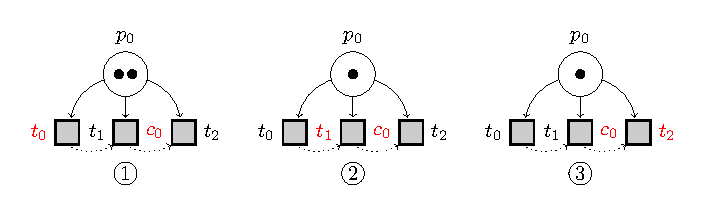
\includegraphics[keepaspectratio=true, width=.8\textwidth]{resid-marking.eps}
  \caption[Computation of the residual marking of a group of
  conflicting transitions.]{Computation of the residual marking for a
    group of conflicting transitions. At \circled{1}
    (resp. \circled{2} and \circled{3}), place $p_0$ holds the
    residual marking for transition $t_0$ (resp. $t_1$ and
    $t_2$). Condition $c_0$ appears in normal font to indicate that
    its current value is \texttt{false}.}
  \label{fig:resid-marking}
\end{figure}

Note that the computation of the residual marking only involves the
consumption phase of the firing process; tokens are withdrawn from
places, but none are generated.

Note also that there is an equivalence between being firable and being
fired at a given state when considering a \textit{top-priority}
transition, i.e. a transition for which there exists no transition
with a higher firing priority.

\paragraph{The state transition relation}

The evolution of the state of a SITPN is \textit{synchronized} with
the rising edge event and the falling edge event of a clock signal.
The rising edge event triggers the marking update, the computation of
time counter reset orders, and the execution of functions. On the
falling edge of the clock signal, the value of conditions are
updated. As the SITPN structure does not hold the link between Boolean
expressions computed over \vhdl{} signals and conditions, the update
of condition values is represented by the injection of fresh Boolean
values coming from an environment. Moreover, the falling edge event
triggers the evolution of the time counter values; values are
incremented, reset, or stalling in the case where a time counter has
reached the upper bound of its associated time interval. Finally, all
actions associated with marked places are
activated. Figure~\ref{fig:sitpn-state-exec} gives an example of the
evolution of the state of a given SITPN through one clock cycle,
happening in the middle of other clock cycles.

\begin{figure}[H]
  \centering
  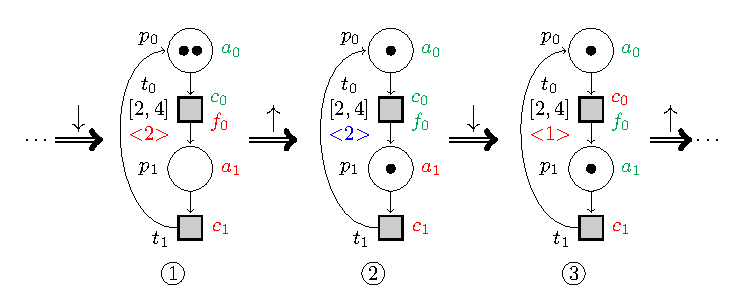
\includegraphics[keepaspectratio=true, width=.8\textwidth]{sitpn-state-evol.eps}
  \caption[Evolution of an SITPN over one clock cycle.]{The evolution
    of a SITPN over one clock cycle. Conditions (i.e. $c_0$ and $c_1$)
    appear in bold font when \texttt{true}; actions (i.e. $a_0$ and
    $a_1$) and functions ($f_0$) appear in bold font when
    activated/executed; time counters appear between diamond brackets,
    and are represented between inverted brackets when they are
    subject to a reset order.}
  \label{fig:sitpn-state-exec}
\end{figure}

In Figure~\ref{fig:sitpn-state-exec}, from Step~1 to Step~2, the
rising edge of the clock signal triggers the firing of transition
$t_0$. As transition $t_0$ is firable and is not in effective conflict
with other transitions, $t_0$ is fired: one token is consumed in place
$p_0$ and one token is produced in place $p_1$. Also, function $f_0$
is executed at the occurrence of the rising edge of the clock signal,
and thus, $f_0$ appears in bold font at Step~2. Consequently to the
firing of $t_0$, a reset order is sent to the time counter of $t_0$,
and it appears between inverted brackets at Step~2. From Step~2 to
Step~3, the falling edge updates the action activation status: $a_0$
stays activated as place $p_0$ is still marked; $a_1$ becomes newly
activated as place $p_1$ just received a token. Time counters are
updated: $t_0$'s time counter is set to zero as the transition
previously received a reset order. However, as $t_0$ is still enabled
by the new marking, its time counter is incremented. Thus, the
resulting time counter value at Step~3 is of one (i.e. result of reset
plus increment). Also, the environment provides a new value to each
condition. As a consequence, condition $c_0$ takes the value
\texttt{false} and condition $c_1$ keeps the same value.

We formalize the evolution of a SITPN state synchronized with the
events of a clock signal with the following state transition relation:

\begin{definition}[SITPN state transition]
  \label{def:semantics}
  For a given $sitpn\in{}SITPN$, the SITPN state transition relation
  $\rightarrow\subseteq{}(\mathbb{N}\rightarrow\mathcal{C}\rightarrow\mathbb{B})\times{}\mathbb{N}\times{}S(sitpn)\times{}\{\uparrow,\downarrow\}\times{}S(sitpn)$
  is noted as follows $E_c,\tau\vdash{}s\xrightarrow{clk}s'$, where
  $E_c\in\mathbb{N}\rightarrow\mathcal{C}\rightarrow\mathbb{B}$ is an
  environment that maps the conditions of $sitpn$ to a Boolean value
  at a given clock count, $\tau\in\mathbb{N}$ is the current clock
  count, $s,s'\in{}S(sitpn)$ are two states of $sitpn$ and
  $clk\in\{\uparrow,\downarrow\}$ is a clock event. The relation is
  defined by the two following rules:
  
  \begin{itemize}
  \item
    $\forall{}E_c\in\mathbb{N}\rightarrow\mathcal{C}\rightarrow\mathbb{B}$,
    $\forall\tau\in\mathbb{N}$, $\forall{}s,s'\in{}S(sitpn)$, we have
    $E_c,\tau\vdash{}s\xrightarrow{\uparrow}s'$, where
    $s=<M,I,reset_t,ex,cond>$ and $s'=<M',I,reset_t',ex',cond>$, if:
    \begin{enumerate}
    \item\label{it:new-marking} $M'$ is the new marking resulting
      from
      the firing of all the transitions contained in $Fired(s)$, i.e.:
      \begin{equation*}
        \forall{}p\in{}P,~M'(p)=M(p)-\sum\limits_{t\in{}Fired(s)}pre(p,t)+\sum\limits_{t\in{}Fired(s)}post(t,p).
      \end{equation*}
      
    \item\label{it:reset-order} A time transition receives a reset
      order if it is fired at state $s$, or, if there exists a place
      $p$ connected to $t$ by a \texttt{basic} or \texttt{test arc}
      and at least one output transition of $p$ is fired and the
      transient marking of $p$ disables $t$; no reset order is sent
      otherwise:
      \begin{equation*}
        \begin{split}
          \forall{}t\in{}T_i,&~t\in{}Fired(s) \\
                             &\lor\big(\exists{}p\in{}P,\omega\in\mathbb{N}^{*}, \\
                             &\quad\quad{}[pre(p,t)=(\omega,\mathtt{basic})\lor{}pre(p,t)=(\omega,\mathtt{test})] \\
                             &\quad\quad\land\sum\limits_{t_i\in{}Fired(s)}pre(p,t_i)>0 \\
                             &\quad\quad\land{}M(p)-\sum\limits_{t_i\in{}Fired(s)}pre(p,t_i)<\omega\big)\\
                             & \Rightarrow{}reset'_t(t)=\mathtt{true}~and~reset'_t(t)=\mathtt{false}~otherwise.  \\
        \end{split}
      \end{equation*}
      
    \item\label{it:exec-fun} All functions associated with at least one fired transition are executed, i.e:
      \begin{equation*}
        \forall{}f\in{}\mathcal{F},~ex'(f)=\sum\limits_{t\in{}Fired(s)}\mathbb{F}(t,f).
      \end{equation*}
    \end{enumerate}
    
  \item
    $\forall{}E_c\in\mathbb{N}\rightarrow\mathcal{C}\rightarrow\mathbb{B}$,
    $\forall\tau\in\mathbb{N}$, $\forall{}s,s'\in{}S(sitpn)$, we have
    $E_c,\tau\vdash{}s\xrightarrow{\downarrow}s'$, where
    $s=<M,I,reset_t,ex,cond>$ and $s'=<M,I',reset_t,ex',cond'>$, if:
    \begin{enumerate}[resume]
    \item\label{it:cond-env} $cond'$ is the function giving the
      (Boolean) values of conditions that are extracted from the
      environment $E_c$ at the clock count
      $\tau$, i.e.:
      \begin{equation*}
        \forall{}c\in{}\mathcal{C},~cond'(c)=E_c(\tau,c).
      \end{equation*}
      
    \item\label{it:activate-actions} All the actions associated
      with at least one
      marked place in the marking $M$ are activated, i.e.:
      \begin{equation*}
        \forall{}a\in{}\mathcal{A},~ex'(a)=\sum\limits_{M(p)>0}\mathbb{A}(p,a).
      \end{equation*}
    \item\label{it:reset-counters} All the time transitions that are
      sensitized by the marking $M$ and received the order to reset
      their time intervals, have their time counter reset and
      incremented, i.e.:
      \begin{equation*}
        \forall{}t\in{}T_i,~t\in{}Sens(M)\land{}reset_t(t)=\mathtt{true}
        \Rightarrow{}I'(t)=1.
      \end{equation*}
      
    \item\label{it:inc-counters} All the time transitions that are
      sensitized by the marking $M$, and
      did not receive a reset order, increment their time counters if time counters are still active, i.e.:
      \begin{equation*}
        \begin{split}
          \forall{}t\in{}T_i,~&t\in{}Sens(M)\land{}reset_t(t)=\mathtt{false}\land{}[I(t)\le{}u(I_s(t))\lor{}u(I_s(t))=\infty]\\
                              & \Rightarrow{}I'(t)=I(t)+1. \\
        \end{split}
      \end{equation*}
    \item\label{it:locked-counters} All the time transitions
      verifying the same
      conditions as above, but with locked counters, keep having locked counters (values are stalling), i.e.:        
      \begin{equation*}
        \begin{split}
          \forall{}t\in{}T_i,~&t\in{}Sens(M)\land{}reset_t(t)=\mathtt{false}\land{}I(t)>{}u(I_s(t))\land{}u(I_s(t))\neq\infty\\
                              & \Rightarrow{}I'(t)=I(t).\\
        \end{split}
      \end{equation*}
      
    \item\label{it:reset-not-sens} All the time transitions disabled by the marking $M$ have their time counters set to zero, i.e.:
      \begin{equation*}
        \forall{}t\in{}T_i,~t\notin{}Sens(M)\Rightarrow{}I'(t)=0.
      \end{equation*}
    \end{enumerate}
    
  \end{itemize}
\end{definition}

Premises~\ref{it:new-marking} to \ref{it:exec-fun} describe the SITPN
state evolution at the rising edge of the clock signal.
Premise~\ref{it:new-marking} corresponds to the marking update. The
computation of the new marking uses the set of fired transitions at
state $s$, i.e. $Fired(s)$. Premise~\ref{it:exec-fun} deals with the
update of the function execution status. Premise~\ref{it:reset-order}
computes the reset orders for time transitions. There are two cases
where a time transition receives the order to reset its time
counter. First, if the transition is one of the fired transitions at
state $s$, then its time counter must be reset on the next falling
edge. Second, if the transition is disabled in a \emph{transient}
manner, then its time counter must also be reset.

Premises~\ref{it:cond-env} to \ref{it:reset-not-sens} describe the
SITPN state evolution at the falling edge of the clock
signal. Premises~\ref{it:cond-env} and \ref{it:activate-actions} deal
with the update of condition values and the activation status of
actions. Note that in Premise~\ref{it:activate-actions} (and also in
Premise~\ref{it:exec-fun}), the sum expression corresponds to the
Boolean sum expression, i.e. the application of the \texttt{or}
operator over the elements of the iterated
set. Premises~\ref{it:reset-counters}, \ref{it:inc-counters},
\ref{it:locked-counters} and \ref{it:reset-not-sens} focus on the
update of time counter values.  In Premise~\ref{it:inc-counters} of
the SITPN semantics, the \emph{active} time counters refer to the time
counters that have not yet overreached the upper bound of their
associated time interval. Of course, a time counter is always active
when the upper bound is infinite. In Premise~\ref{it:locked-counters},
the \emph{locked} time counters refer to the time counters that have
overreached the upper bound of their associated time interval. Of
course, time counters can never be locked in the presence of an
infinite upper bound. In Premises~\ref{it:inc-counters} and
\ref{it:locked-counters}, for a given time interval $i$, $u(i)$
denotes the upper bound of the time interval, and $l(i)$ denotes the
lower bound of the time interval.\\

To give a small-step execution semantics to a SITPN model, we have
defined an execution relation that binds a given SITPN model to an
execution trace, i.e. a time-ordered list of states. The execution
trace is built for a given number of clock cycles, starting from the
initial state of the SITPN model. The execution relation is
implemented in \coq{} by the \texttt{SitpnFullExec} inductive
type\footnote{\url{https://github.com/viampietro/ver-hilecop/blob/master/sitpn/SitpnSemantics.v}}. The
initial state of a SITPN model is formally defined as follows:

\begin{definition}[Initial state]
  \label{def:sitpn-init-state}
  For a given $sitpn\in{}SITPN$, $s_0\in{}S(sitpn)$ is the initial
  state of $sitpn$, such that
  $s_0=<M_0,O_\mathbb{N},O_\mathbb{B},O_\mathbb{B},O_\mathbb{B}>$,
  where $M_0$ is the initial marking of the SITPN, $O_\mathbb{N}$ is a
  function that always returns 0, $O_\mathbb{B}$ is a function that
  always returns \texttt{false}.
\end{definition}

\subsection{Well-definition of a SITPN}
\label{sec:sitpn-wd}

The synchronous execution semantics of SITPNs implies that all
transitions are fired at the same time. In
Figure~\ref{fig:double-consum}, transitions $t_0$ and $t_1$ are both
firable before the rising edge event. As no priority relation is drawn
between the two conflicting transitions, they are both fired at the
occurrence of the event. The system acts as if two tokens were
available in place $p_0$, one for the firing of $t_0$ and another for
the firing of $t_1$.

\begin{figure}[H]
  \centering
  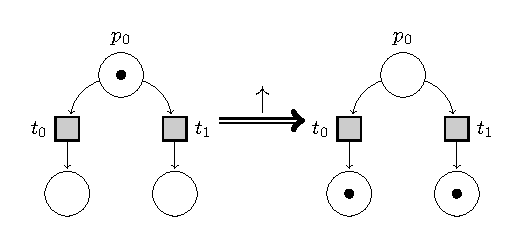
\includegraphics[keepaspectratio=true, width=.5\textwidth]{double-consum.eps}
  \caption[Double consumption of token in a SITPN.]{Double consumption
    of one token in a SITPN. On the left side, the current marking
    before the firing of $t_0$ and $t_1$; on the right side, the
    marking resulting of the firing of $t_0$ and $t_1$. The arrow
    indicates the occurrence of a rising edge that triggers the firing
    process.}
  \label{fig:double-consum}
\end{figure}

In the context of a SITPN, a branching like the one of
Figure~\ref{fig:double-consum}, normally interpreted as a disjunctive
branching, takes the semantics of a conjunctive branching if no
priority are specified between the conflicting transitions. To avoid
the phenomenon of ``double consumption'' of tokens, we enforce the
resolution of any structural conflict by means of mutual exclusion or
through the application of priorities. This policy about the
resolution of structural conflicts is part of the definition of a
\emph{well-defined} SITPN. We must be able to decide which transition
in a conflicting pair will be fired when the conflict becomes
effective. Thus, we give place-centered definition of a group of
transitions in conflict:

\begin{definition}[Conflicting group of transitions]
  \label{def:cgroup}
  For a given $sitpn\in{}SITPN$, the conflicting transitions of a
  given place $p$, noted $conflict(p)$, are all transitions related to
  $p$ with a \texttt{basic} place-transition arc,
  i.e.
  $conflict(p)=\{t\in{}T~\vert~\exists{}\omega\in\mathbb{N}^{*},~pre(p,t)=(\omega,\mathtt{basic})\}$.
\end{definition}

This view of a conflict group reflects the place-centered view of
conflicts as implemented in the \vhdl{} code generated by the
model-to-text transformation.  Figure~\ref{fig:conflict-groups} shows
the conflict group related to place $p_0$ and $p_1$, namely:
$\{t_0,t_3\}$ and $\{t_1,t_4\}$.

\begin{figure}[H]
  \centering
  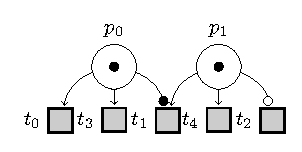
\includegraphics[keepaspectratio,width=.3\linewidth]{conflict-groups.eps}
  \caption[An example of two separate conflict groups.]{An example of
    two separate conflict groups, namely: $\{t_0,t_3\}$ and
    $\{t_1,t_4\}$.}
  \label{fig:conflict-groups}
\end{figure}

In a well-defined SITPN, all conflicts in a conflict group must be
considered, i.e. for all pair of transitions in the group the conflict
must be solved. When the conflict between a pair of transitions
becomes effective, there are two ways to be sure that only one
transition will be fired. The first way is to define a firing order
through a priority relation. The second way is to use a mean of mutual
exclusion. A mean of mutual exclusion ensures that the two transitions
of a conflicting pair will never be firable at the same time. We only
consider two ways of mutual exclusion, namely: mutual exclusion with
complementary conditions and mutual exclusion with inhibitor arcs.

\begin{definition}[Mutual exclusion with complementary conditions]
  \label{def:mutex-conds}
  Given two conflicting transitions $t_0$ and $t_1$, $t_0$ and $t_1$
  are in mutual exclusion with complementary conditions if there
  exists $c\in\mathcal{C}$ such that
  $(\mathbb{C}(t_0,c)=1\land{}\mathbb{C}(t_1,c)=-1)$ or
  $(\mathbb{C}(t_0,c)=-1\land{}\mathbb{C}(t_1,c)=1)$.
\end{definition}

\begin{definition}[Mutual exclusion with an inhibitor arc]
  \label{def:mutex-inhib} Given two conflicting transitions $t_0$ and
  $t_1$, $t_0$ and $t_1$ are in mutual exclusion with an inhibitor arc
  if there exists $p\in{}P$ and $\omega\in{}\mathbb{N}^{*}$ such that
  $(pre(p,t_0)=(\omega,\mathtt{basic})\lor{}pre(p,t_0)=(\omega,\mathtt{test}))\land{}pre(p,t_1)=(\omega,\mathtt{inhib})$
  or
  $(pre(p,t_1)=(\omega,\mathtt{basic})\lor{}pre(p,t_1)=(\omega,\mathtt{test}))\land{}pre(p,t_0)=(\omega,\mathtt{inhib})$.
\end{definition}

Figure~\ref{fig:mutex} illustrates the two means of mutual exclusion
that can be applied to solve a conflict between two transitions.

\begin{figure}[H]
  \centering
  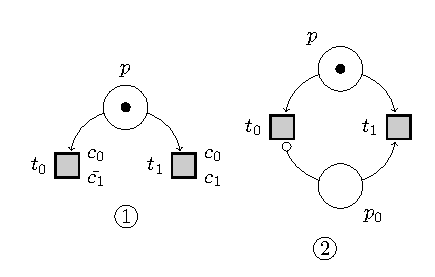
\includegraphics[keepaspectratio,width=.45\linewidth]{mutex.eps}
  \caption[Examples of conflicting transitions in mutual exclusion.]{
    Examples of conflicting transitions in mutual exclusion. At
    \circled{1}, an example of mutual exclusion with complementary
    conditions; at \circled{2}, an example of mutual exclusion with an
    inhibitor arc.}
  \label{fig:mutex}
\end{figure}

In Figure~\ref{fig:mutex}, in situation \circled{1}, condition $c_1$
is associated to $t_1$ and the complementary condition is associated
to $t_0$ thus creating the mutual exclusion. In situation \circled{2},
the arcs $(p_0,t_0)$ and $(p_0,t_1)$ ensure the mutual exclusion
between transitions $t_0$ and $t_1$. Note that in the structure of
mutual exclusion with an inhibitor arc, the weight of the inhibitor
arc and of the one of the basic or test arc must be the same;
otherwise, the mutual exclusion is not effective.\\

\noindent{}A well-defined SITPN is defined as follows:

\begin{definition}[Well-defined SITPN]\label{def:wd-sitpn}
  A given $sitpn\in{}SITPN$ is well-defined if:
  \begin{itemize}
  \item $T\neq\emptyset$, the set of transitions is not empty.
  \item $P\neq\emptyset$, the set of places is not empty.
  \item There is no isolated place, i.e. a place that has neither
    input nor output transitions:\\
    $\nexists{}p\in{}P,~input(p)=\emptyset\wedge{}output(p)=\emptyset$,
    where $input(p)$ (resp. $output(p)$) denotes the set of input
    (resp. output) transitions of $p$.
  \item There is no isolated transition, i.e. a transition that has
    neither
    input nor output places:\\
    $\nexists{}t\in{}T,~input(t)=\emptyset\wedge{}output(t)=\emptyset$,
    where $input(t)$ (resp. $output(t)$) denotes the set of input
    (resp. output) places of $t$.
  \item For all conflict group as defined in
    Definition~\ref{def:cgroup}, either all conflicts (i.e. for all
    pair of transitions in the conflict group) are solved by one of
    the mean of mutual exclusion, or, the priority relation is a
    \emph{strict total} order over the transitions of the conflict group.
  \end{itemize}
\end{definition}

If the properties, given in Definition~\ref{def:wd-sitpn}, are not
ensured, they will lead to compile-time errors during the
transformation of a SITPN model into a \vhdl{} design.


%%% Local Variables:
%%% mode: latex
%%% TeX-master: "main"
%%% End:
